% !TEX root = main.tex
\section {Vergleich reaktive \& imperative Anwendung}
\label{section:vergleich_reaktiv_imperativ}
Um zu prüfen, ob Leistungsfähigkeit und Skalierbarkeit einer reaktiven Anwendung tatsächlich die einer traditionellen, imperativen Anwendung
übertrifft, werden in diesem Kapitel beide Ansätze hinsichtlich verschiedener Metriken in einem festen Zeitintervall miteinander verglichen.

\subsection{Implementierung \& Systemaufbau}
\label{section:implementierung}
Die beiden Anwendungen implementieren mit dem Quarkus-Framework jeweils eine simple REST-Schnittstelle mit HTTP-CRUD Methoden
und einer angebundenen PostgreSQL-Datenbank.
Dabei ist vorallem die HTTP-Schicht von Interesse. Die HTTP-Unterstützung von Quarkus basiert auf einem reaktiven, nicht-blockierenden
Unterbau: der Vert.x Engine.
Jede HTTP-Anfrage wird auf einem der \textit{event-loop threads} bzw. \textit{IO threads}
\footnote{Deren Anzahl hängt von der Anzahl der CPU-Kerne ab}
verarbeitet und durch eine Routing-Schicht an den Anwendungscode weitergeleitet.
Je nachdem welcher Ansatz zur Implementierung des jeweiligen HTTP-Endpunktes gewählt wurde,
wird der abzuarbeitende Code dann auf einem blockierenden \textit{worker thread} aus dem \textit{worker thread pool}
\footnote{Auch als \textit{Dispatch} bezeichnet} (Servlet, JAX-RS) oder einem der
\textit{IO threads} (Reactive Routes, Reactive Resteasy) ausgeführt.
Die \textit{IO threads} sind dafür zuständig alle IO-Operationen asynchron auszuführen und die jeweiligen EventListener bzw. Subscriber auszulösen sobald
die Operationen abgeschlossen sind.
\newpage
\begin{figure}[h!]
    \centering
    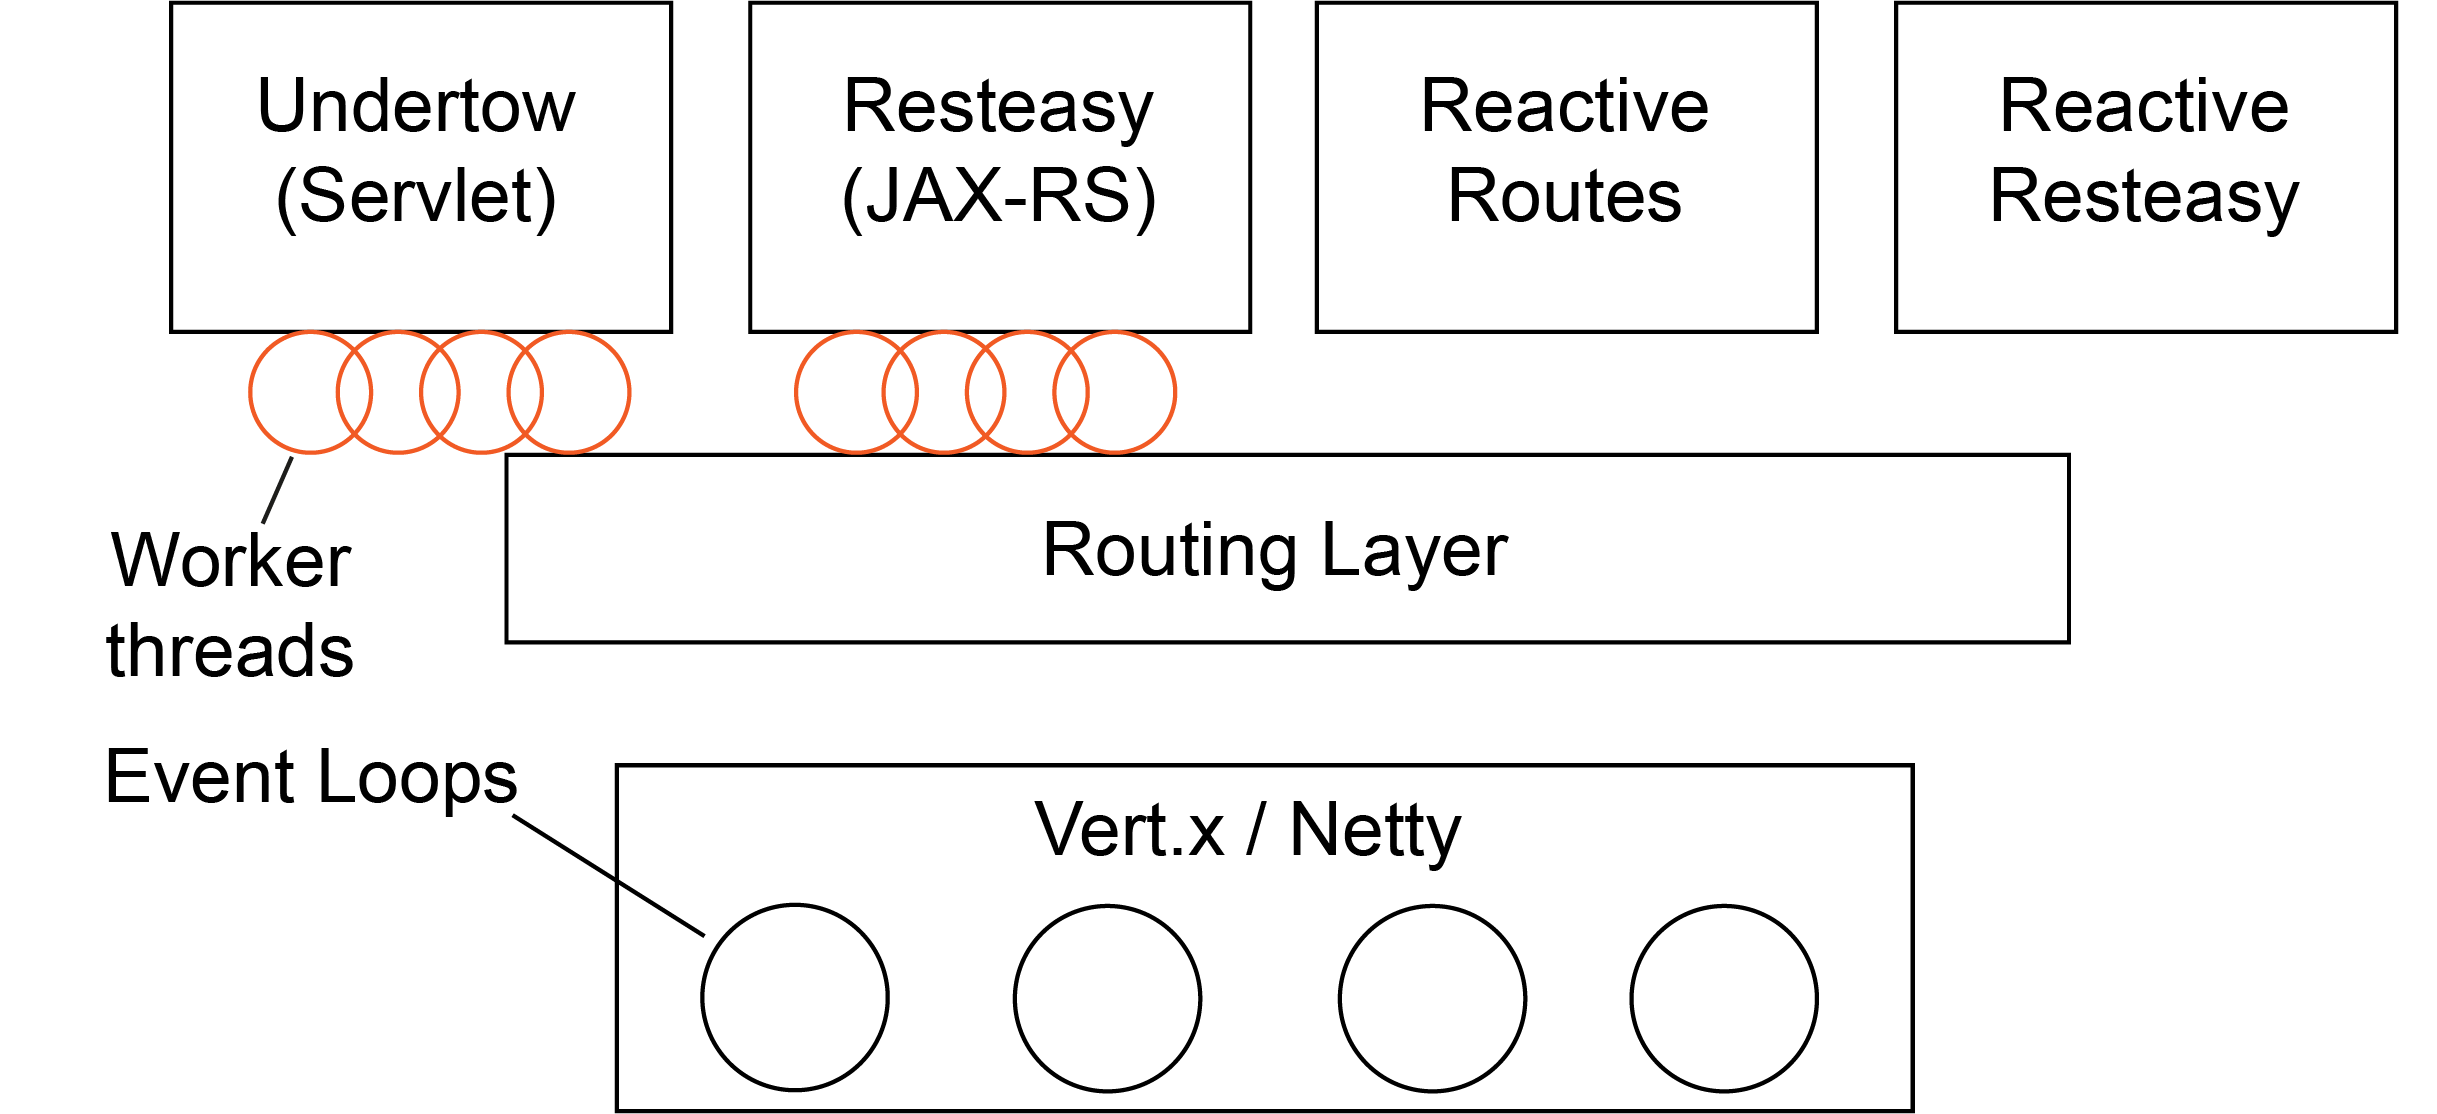
\includegraphics[width=1.0\textwidth]{Quarkus_HTTP_Layer}
    \caption{Quarkus HTTP-Schicht \parencite{QuarkusReactiveRoutes}}
\end{figure}

Damit sich beide Anwendungen nahe an einer realen Java-EE REST-API orientieren, haben
sie (zusätzlich zu den grundlegenden Abhängigkeiten des Quarkus-Frameworks) folgende Projekt-Abhängigkeiten:
\begin{enumerate}
    \item JAX-RS Implementierung
    \item JSON Unterstützung
    \item Datenbanktreiber
    \item JPA Implementierung
\end{enumerate}

Diese Abhängigkeiten wurden vom Quarkus Maven-Repository sowohl in blockierender,
als auch in nicht-blockierender, reaktiver Form bereitgestellt: \parencite{MavenQuarkusIO}
% space between the text and the left/right border of its containing cell is set to 18 pt
\setlength{\tabcolsep}{18pt}
% the height of each row is set to 1.5 relative to its default height
\renewcommand{\arraystretch}{1.5}
\begin{table}[ht!]
    \centering
    \begin{tabular}{| c | c | c |}
        \hline
                         & Blockierend      & Nicht-blockierend (reaktiv) \\
        \hline
        JAX-RS           & Resteasy         & Resteasy Reactive           \\
        \hline
        JSON             & Resteasy-Jackson & Resteasy-Reactive-Jackson   \\
        \hline
        Datenbanktreiber & JDBC-Postgresql  & Reactive-Pg-Client          \\
        \hline
        JPA-/ORM         & Hibernate-ORM    & Hibernate-Reactive          \\
        \hline
    \end{tabular}
    \caption{Tabelle mit den verwendeten Anwendungen beider Applikationen}
    \label{table:dependencies}
\end{table}
Der Projekt-Code dieser Arbeit kann vom Gitlab-Server der Ostfalia unter
\url{//TODO Ostfalia Gitlab link?} eingesehen und abgerufen werden.
\subsection{Testumgebung}
\label{section:testumgebung}
Für die Testumgebung werden zwei Systeme benötigt: der Client-Host und der Server-Host.
Dabei muss es sich um UNIX-Systeme handeln, da eine einige der verwendeten Werkzeuge nur 
auf diesen Systemen verfügbar sind.
Zudem müssen beide Systeme per SSH von einem (idealerweise vorhandenem) dritten System 
\footnote{Dies kann allerdings auch der Client-Host selber sein} 
erreicht werden können, damit dieses den Testablauf in der korrekten Abfolge ausführen kann. 
Der Einfachheit halber empfiehlt es sich, dass sich alle Geräte im gleichen Netzwerk befinden.
Beiden Anwendungen verwenden Version 2 des Quarkus Frameworks. 
Um eine reproduzierbare Anwendungsumgebung und Ressourcenallokation zu ermöglichen, laufen beide Anwendungen auf dem Server-Host in
jeweils in einem Docker-Container mit fest definierten Ressourcen:
\begin{itemize}
    \item Nutzung von 4 CPU-Kernen
    \item 1024 MB RAM
    \item \textit{-Xmx512m} Heap Größe für den Java-Prozess
\end{itemize}

Die jeweiligen Docker-Container für die Postgresql-Datenbank allokieren:
\begin{itemize}
    \item 4 CPU-Kerne
    \item 2048 MB RAM
\end{itemize}

Die Anwendung, die auf dem Client-Host die \textit{work load} für die beiden zu testenden Anwendungen generiert,
 nutzt in dieser Testumgebung 4 Threads.
\footnote{Alle genannten Ressourcen-Parameter können im Verzeichnis \textit{/scripts/qDup} des Quellcodeverzeichnisses eingesehen und
angepasst werden.}
Welche Laufzeitumgebungen und Tools für diesen Versuch auf den jeweiligen Hosts vorhanden sein müssen, 
wird in der Readme.md Datei des Projektverzeichnisses genau beschrieben und auch im nachfolgenden Kapitel durch eine Grafik dargestellt.
//TODO: Anwendungen testen nach Umstellung auf Quarkus V2 und Jvm Heap auf 512 mb setzen
Die vom Autor genutzten Client- und Server-Host Systeme zur Durchführung der Tests haben die folgenden Systemspezifikationen:

\begin{table}[ht!]
    \centering
    \begin{tabular}{| c | c |}
        \hline
        Server-Host TODO\\
        \hline
        CPU's           & Resteasy         \\
        \hline
        RAM            & Resteasy-Jackson \\
        \hline
        Speicher & JDBC-Post        \\
        \hline
        Betriebssystem         & Hibernate-ORM    \\
        \hline
        Kernel & \\
        \hline
    \end{tabular}
    \caption{Tabelle mit den verwendeten Anwendungen beider Applikationen}
    \label{table:system_host}
\end{table}

\begin{table}[ht!]
    \centering
    \begin{tabular}{| c | c |}
        \hline
        Client-Host\\
        Hardware & Acer Aspire VN7-591G \\
        \hline
        CPU      & Intel® Core™ i5-4210H CPU @ 2.90GHz × 4          \\
        \hline
        RAM      & 8GB \\
        \hline
        Speicher & 500 GB   \\
        \hline
        Betriebssystem  & Fedora 34 (Workstation Edition)   \\
        \hline
        Kernel & Linux version \verb|5.12.13-300.fc34.x86_64| \\
        \hline
    \end{tabular}
    \caption{Systemspezifikationen der verwendeten Client-Maschine}
    \label{table:system_client}
\end{table}

\subsection{Testvorgehen / Testaufbau}
\label{section:vorgehen}
Der im Folgenden erläuterte Versuchsaufbau basiert auf einer, vom Autor erweiterten, Architektur die vom Quarkus-Entwicklerteam 
  zur Erstellung von verschiedenen Benchmarks für den Quarkus Technologie-Stack genutzt wurde. 
  \parencite{QuarkusBlog, QuarkusJohnaohara}

  Um den gesamten Versuchsablauf zu automatisieren und über mehrere Server zu steuern wird ein Tool namens qDup eingesetzt.
  Damit können Shell-Kommandos als Skripte gruppiert, und verschiedenen Hosts je nach Rolle zugewiesen werden.
  Um dem Ablauf korrekt zu steuern, werden Signale definiert die ein Host sendet, und auf die die anderen Hosts warten um ihrerseits
  weitere Skripte auszuführen.
  \footnote{Beispielsweise sollte der Server-Host erst anfangen den Java-Prozess zu überwachen, sobald der Client-Host die \textit{workload}
  generiert und nicht bereits davor}.
  Wie bereits in \ref{section:testumgebung} erwähnt, nutzt qDup SSH um mit den jeweiligen Servern zu kommunizieren.

  Zu Beginn wird auf dem Server-Host das Quellcodeverzeichnis geklont und beide Anwendungen werden gebaut (je nach Test entweder
  .jar oder als native executable). Anschließend wird über ein JavaScript-Skript, welches in der Laufzeitumgebung Node.js läuft, das 
  durchschnittliche Zeitintervall zwischem dem Start einer Anwendung bis zur Verarbeitung der ersten Anfrage gemessen, auch als
  \textit{Mean Start Time to First Request} bezeichnet. 


  
 //TODO: Erklären wie das gesamte System getestet wird, welche Werkzeuge ssh, (wrk2 (warum wrk2,
  latenzmessung im gegensatz zu wrk), top, jbang etc.
docker für reproduzierbare umgebung, lua histogramme dann durch javascript-script zu graphen )
Systemaufbau (Client-Host, Server-Host, User-Host)
Architekturaufbau als Grafik
//eine minute lang http anfragen an zwei Anwendungen, die genau dasselbe machen
was genau gemessen wird (welche Metriken) und wie (mean start time to first request als uber-jar in jvm mode)
diees beeeinflusst werden können und wie diese durch top \& wrk ermittelt werden
Jeden größeren Schritt erklären, Bauen der Anwendungen, Warm-Up (JIT), Workload
//TODO: Grafik zur Visualisierung (Illustrator)
\subsection{Test: Statische Daten}
\label{section:statische_daten}

\subsubsection{Systemablauf}
//TODO: Grafik ähnlich zu Grafik in Implementierung aber mit Threadwechseln und exemplarisch mhrere Threads zeigen
(auch angeben wie Ergebnisse mit komplizierteren Queries aussehen könnten)
\subsubsection{Resultate}

\subsection{Test: Datenbankzugriffe}
\label{section:datenbankzugriffe}

\subsubsection{Systemablauf}
//TODO: Grafik ähnlich zu Grafik in Implementierung aber ohne Threadwechsel dafür Main-Thread mit dahinterliegender Datenbank,
das Nicht BLockieren bzw. Asynchronität verdeutlichen

\subsubsection{Resultate}

//auch erwähnen dss beide paradigmen gemischt werden können, und vert.x dann entweder die anfrage an den worker thread pool dispatched
// (auch mit kosten verbunden)
// oder auf dem io thread ausführt -> muss nicht komplett reaktiv oder blockierend sein x
\subsection{Auswertung}
\label{section:auswertung}